% ORfe - OpenRadioss Workbench for FreeCAD: a short introduction
% Build: pdflatex ORfe_Introduction.tex (twice, for the references)
\documentclass[11pt,a4paper]{article}

\usepackage[utf8]{inputenc}
\usepackage[T1]{fontenc}
\usepackage{lmodern}
\usepackage{microtype}
\usepackage[margin=2.5cm]{geometry}
\usepackage{booktabs}
\usepackage{tabularx}
\usepackage{enumitem}
\usepackage{xcolor}
\usepackage{listings}
\usepackage{caption}
\usepackage{tikz}
\usetikzlibrary{arrows.meta,positioning,fit}
\usepackage[colorlinks=true,linkcolor=blue!50!black,urlcolor=blue!50!black]{hyperref}

\lstset{basicstyle=\ttfamily\small,columns=fullflexible,keepspaces=true,
        backgroundcolor=\color{black!4},frame=none,xleftmargin=1em,breaklines=true}
\setlist{itemsep=2pt,topsep=4pt}
\emergencystretch=1.5em

\newcommand{\cmd}[1]{\textsf{\textbf{#1}}}
\newcommand{\unit}[1]{\,\mathrm{#1}}

\title{ORfe -- OpenRadioss Workbench for FreeCAD\\[4pt]
       \large A short introduction}
\author{Nicholas Herrmann}
\date{November 2026 \quad (workbench version 0.0.1)}

\begin{document}
\maketitle

\begin{abstract}
\noindent ORfe brings the explicit finite element solver OpenRadioss into FreeCAD. It adds
\emph{OpenRadioss} as a solver of the FEM workbench, next to CalculiX, Elmer, Mystran and Z88,
so an analysis set up in the usual way (mesh, material, constraints) can be solved as an explicit
dynamic problem and post-processed in FreeCAD. A separate \emph{OpenRadioss} workbench edits
LS-DYNA format input decks (\texttt{.k} files) with a keyword editor and templates, and runs them.
This note explains what the workbench does, how to install and use it, how it was tested, and its
current limitations.
\end{abstract}

\section{Why an explicit solver in FreeCAD?}

The solvers bundled with FreeCAD FEM are implicit: well suited for static and modal analyses, but
expensive for short, highly nonlinear events such as impacts, drop tests, crushing or forming.
Explicit codes integrate the equations of motion with very small time steps and need no global
stiffness matrix, which makes them robust for contact, large deformation and failure. OpenRadioss
is an industry-proven explicit solver (AGPL) that reads the widely used LS-DYNA keyword format
natively. ORfe connects the two: FreeCAD provides geometry, meshing and post-processing,
OpenRadioss the explicit solution.

\paragraph{Note on OpenRadioss and OpenCourant.}
In October 2026 the OpenRadioss project was discontinued and its GitHub repository removed. The
community continues the code as \textbf{OpenCourant}
(\url{https://github.com/OpenCourant/OpenCourant}), with ready-to-run Linux and Windows
releases. The release layout and the executable names in \texttt{exec/} are unchanged, so ORfe
works with OpenCourant as it is; ``OpenRadioss'' in this text means either.

\section{Installation}

\begin{enumerate}
  \item Install FreeCAD 1.0 or newer (tested with 1.0.0 and the 1.1.4 Flatpak).
  \item Download a solver release from the OpenCourant releases page (on Linux
        \texttt{OpenCourant\_\allowbreak linux64.zip}) and unpack it to \texttt{\textasciitilde/OpenRadioss},
        the default location. Another folder can be chosen in the \cmd{Run OpenRadioss} dialog;
        the FEM solver uses the same setting.
  \item Put the workbench into FreeCAD's \texttt{Mod} directory and restart FreeCAD:
\begin{lstlisting}
git clone https://github.com/CalzitPLA/ORfe ~/.local/share/FreeCAD/Mod/ORfe
# Flatpak: ~/.var/app/org.freecad.FreeCAD/data/FreeCAD/Mod/ORfe
\end{lstlisting}
\end{enumerate}
Inside the FreeCAD Flatpak the solver binaries miss two host libraries (\texttt{libcrypt.so.1},
\texttt{libapr-1.so.0}); ORfe copies them automatically to
\texttt{<solver>/\allowbreak extlib/\allowbreak flatpak\_compat} before the first run.

\section{Workflow 1: OpenRadioss as a FEM workbench solver}

This is the quickest way in for FreeCAD FEM users. Set up an analysis as for CalculiX, then choose
\cmd{Solve $\rightarrow$ Solver OpenRadioss} and run it with \cmd{Run solver calculations} (or by
double-clicking the solver). Figure~\ref{fig:pipeline} shows what happens behind the scenes.

\begin{figure}[ht]
\centering
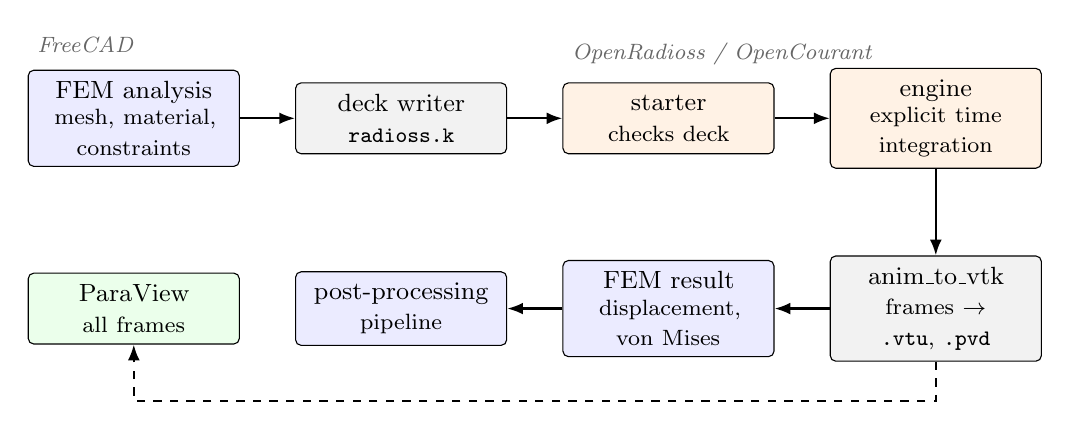
\begin{tikzpicture}[
    box/.style={draw,rounded corners=2pt,fill=#1,minimum height=9mm,align=center,
                font=\small,inner sep=4pt,text width=24mm},
    box/.default=black!5,
    arr/.style={-{Latex[length=2mm]},thick},
    node distance=5mm and 7mm]
  \node[box=blue!8]   (fc)   {FEM analysis\\ \footnotesize mesh, material,\\ \footnotesize constraints};
  \node[box,right=of fc]   (deck) {deck writer\\ \footnotesize \texttt{radioss.k}};
  \node[box=orange!10,right=of deck] (st) {starter\\ \footnotesize checks deck};
  \node[box=orange!10,right=of st]   (en) {engine\\ \footnotesize explicit time\\ \footnotesize integration};
  \node[box,below=11mm of en]  (vtk)  {anim\_to\_vtk\\ \footnotesize frames $\rightarrow$ \texttt{.vtu}, \texttt{.pvd}};
  \node[box=blue!8,left=of vtk] (res)  {FEM result\\ \footnotesize displacement,\\ \footnotesize von Mises};
  \node[box=blue!8,left=of res] (pp)   {post-processing\\ \footnotesize pipeline};
  \node[box=green!8,left=of pp] (pv)   {ParaView\\ \footnotesize all frames};
  \draw[arr] (fc) -- (deck); \draw[arr] (deck) -- (st); \draw[arr] (st) -- (en);
  \draw[arr] (en) -- (vtk);  \draw[arr] (vtk) -- (res); \draw[arr] (res) -- (pp);
  \draw[arr,dashed] (vtk.south) |- ++(0,-5mm) -| (pv.south);
  \node[font=\footnotesize\itshape,text=black!60,above=1mm of fc.north west,anchor=south west] {FreeCAD};
  \node[font=\footnotesize\itshape,text=black!60,above=1mm of st.north west,anchor=south west] {OpenRadioss / OpenCourant};
\end{tikzpicture}
\caption{Solving a FEM analysis with OpenRadioss. Blue: FreeCAD objects, orange: solver steps.}
\label{fig:pipeline}
\end{figure}

The last frame is loaded as a regular FEM mechanical result (displacements, von Mises and principal
stresses, like CalculiX results) plus a post-processing pipeline. All frames stay in the working
directory as \texttt{radioss.pvd} for ParaView.

\paragraph{Solver properties.}
OpenRadioss is an explicit dynamic solver; the properties of the solver object control the time
integration (Table~\ref{tab:props}).

\begin{table}[ht]
\centering\small
\begin{tabularx}{\linewidth}{@{}lX@{}}
\toprule
Property & Meaning \\
\midrule
\texttt{EndTime} & Simulated time (default $0.01\unit{s}$). Explicit time steps are tiny, so keep it short. \\
\texttt{LoadCurve} & \emph{Ramp}: loads grow linearly from 0 over \texttt{EndTime} (quasi-static);
                     \emph{Constant}: loads act fully from the start (impact-like). \\
\texttt{OutputFrames} & Number of result frames written. \\
\texttt{MassScalingMicroseconds} & 0 = off; otherwise mass is added so that the time step stays at
                     least this value (e.g.\ 0.2\,\textmu s). Much faster, but check the added mass in the listing. \\
\texttt{Threads} & Threads for starter and engine. \\
\texttt{AdditionalKeywords} & A text document whose keywords are appended to the deck, e.g.\ from the Keyword Editor. \\
\bottomrule
\end{tabularx}
\caption{Properties of the \emph{SolverOpenRadioss} object.}
\label{tab:props}
\end{table}

\paragraph{What is translated.}
Volume meshes (tetra4, tetra10, hexa8, penta6, pyra5; second-order hexa, penta and pyramid elements
are reduced to their corner nodes) and face meshes with a shell thickness; linear elastic materials,
several via references; fixed and displacement constraints (fixed components), force, pressure and
self weight. Other constraints are reported and ignored. The deck uses consistent
mm\,/\,t\,/\,s\,/\,N\,/\,MPa units.

\section{Workflow 2: the OpenRadioss workbench (keyword decks)}

For models beyond the FEM translation (contacts, other materials, initial velocities, \dots) the
\emph{OpenRadioss} workbench works directly on LS-DYNA keyword text:

\begin{description}[font=\sffamily\bfseries,leftmargin=1em]
  \item[Create Basic .k File] adds a small runnable deck (one shell element) as a text object.
  \item[Keyword Editor] browses 219 keywords with their card layouts, field help and links to the
        Radioss documentation, fills in card fields and caches the generated keywords;
        \emph{Update .k File} writes them into the document. A \emph{Templates} menu starts from
        ready-made keyword sets.
  \item[Template Editor] creates, edits, reorders and deletes templates with a live preview.
        User templates are stored in \texttt{<FreeCAD user data>/ORfemn/templates.json}.
  \item[Run OpenRadioss] runs starter, engine and the VTK conversion in the background with a live
        log and a Stop button, then loads the result into FEM post-processing.
  \item[Export LS-DYNA .k File] saves a keyword text object to disk.
\end{description}
Both workflows meet in the \texttt{AdditionalKeywords} property: keywords written in the editor
can extend a deck generated from a FEM analysis.

\section{Testing}

The workbench was tested on Debian 13 with FreeCAD 1.0.0 (Debian package), FreeCAD 1.1.4 (Flatpak)
and OpenCourant \texttt{latest-20261011}:
\begin{itemize}
  \item 43 unit and integration tests (\texttt{python tests/tests.py}): \texttt{.k} formatting,
        templates, deck writer, result conversion, and two real solver runs. All pass.
  \item Headless FreeCAD script: a cantilever analysis (Gmsh mesh, steel, fixed face, tip force)
        gets an OpenRadioss solver, writes the deck, solves through the FEM solver framework and
        loads the result; the document is saved and restored with the solver object.
  \item GUI smoke test (FreeCAD 1.1.4): workbench activation, all eight commands, Create Radioss
        Model, Create Basic .k File, Keyword and Template Editor dialogs, and the
        \emph{Solver OpenRadioss} entry in the FEM workbench toolbar.
\end{itemize}
Testing found one incompatibility, now fixed: FreeCAD~1.1 changed the arguments of
\texttt{ObjectsFem\allowbreak.makePostVtkResult}, so loading results failed there.

\paragraph{Accuracy check.}
Table~\ref{tab:beam} compares the tip deflection of a steel cantilever
($100\times10\times10\unit{mm}$, $E=210\,000\unit{MPa}$, $F=100\unit{N}$, ramp load over
$10\unit{ms}$) with beam theory ($0.192\unit{mm}$ including shear) and with CalculiX on the same
kind of mesh. Hexahedra and linear tetrahedra agree with the reference solutions. With the
solver's 10-node tetrahedron the beam deflects about $35\,\%$ more than with CalculiX, and the
starter reports only $0.70$ of the physical mass for every tetra10 mesh tried. The deck's tetra10 node order was checked
(every other midside order is rejected by the starter), so this behaviour comes from the solver
element, not from the translation. Until this is understood, use hexahedra or a fine tetra4 mesh
for quantitative results.

\begin{table}[ht]
\centering\small
\begin{tabular}{@{}llrrr@{}}
\toprule
Mesh & Element & OpenCourant [mm] & CalculiX [mm] & Difference \\
\midrule
$40\times10\times10$, $8\times2\times2$ & hexa8 & 0.01224 & -- & $+0.4\,\%$ vs.\ beam \\
Gmsh, 4\,mm & tetra4  & 0.1329 & 0.1307 & $+1.7\,\%$ \\
Gmsh, 2\,mm & tetra4  & 0.1827 & 0.1679 & $+8.8\,\%$ \\
Gmsh, 4\,mm & tetra10 & 0.2592 & 0.1908 & $+36\,\%$ \\
\bottomrule
\end{tabular}
\caption{Tip deflection of the cantilever. Linear tetrahedra are too stiff in both codes
(shear locking), so they are compared with CalculiX, not with beam theory. The tetra10 value was
computed without mass scaling.}
\label{tab:beam}
\end{table}

\section{Limitations and tips}

\begin{itemize}
  \item Explicit means \emph{dynamic}: a ramp over several periods of the lowest eigenmode gives a
        quasi-static answer; a constant load gives an impact response with oscillations.
  \item Mass scaling speeds runs up a lot, but with quadratic tetrahedra it can easily double the
        mass; check \emph{MASS ADDED} in \texttt{radioss\_0001.out}.
  \item Only linear elastic materials and the constraints listed above are translated; anything
        else can be added as keywords through \texttt{AdditionalKeywords}.
  \item For bending with hexahedra use at least two elements through the thickness.
  \item Tested on Linux; the code also handles Windows and arm64 executable names, but these
        platforms are untested.
\end{itemize}

\section{Source, license and feedback}

Source code, issue tracker and this document: \url{https://github.com/CalzitPLA/ORfe}.
ORfe is free software under the GNU Lesser General Public License, version~2.1 or later, like
FreeCAD itself. OpenRadioss and OpenCourant are separate programs under the AGPL; ORfe only runs
their executables. Feedback is welcome on the FreeCAD forum (FEM section) or as GitHub issues.

\end{document}
